During this third year another four territorial PoPs have been raised and made operative, amounting to a total of 11 territorial and the concentration one (Telvent -Barcelona) being operational. \figurename~\ref{fig:pop_weathermap} shows their distribution on the map. So far all the territorial PoPs are connected to the concentration one via XOC connections\footnote{The prices can be found at \url{http://www.xarxaoberta.cat/en/prices}.}.

\begin{figure}[H]
  \centering
  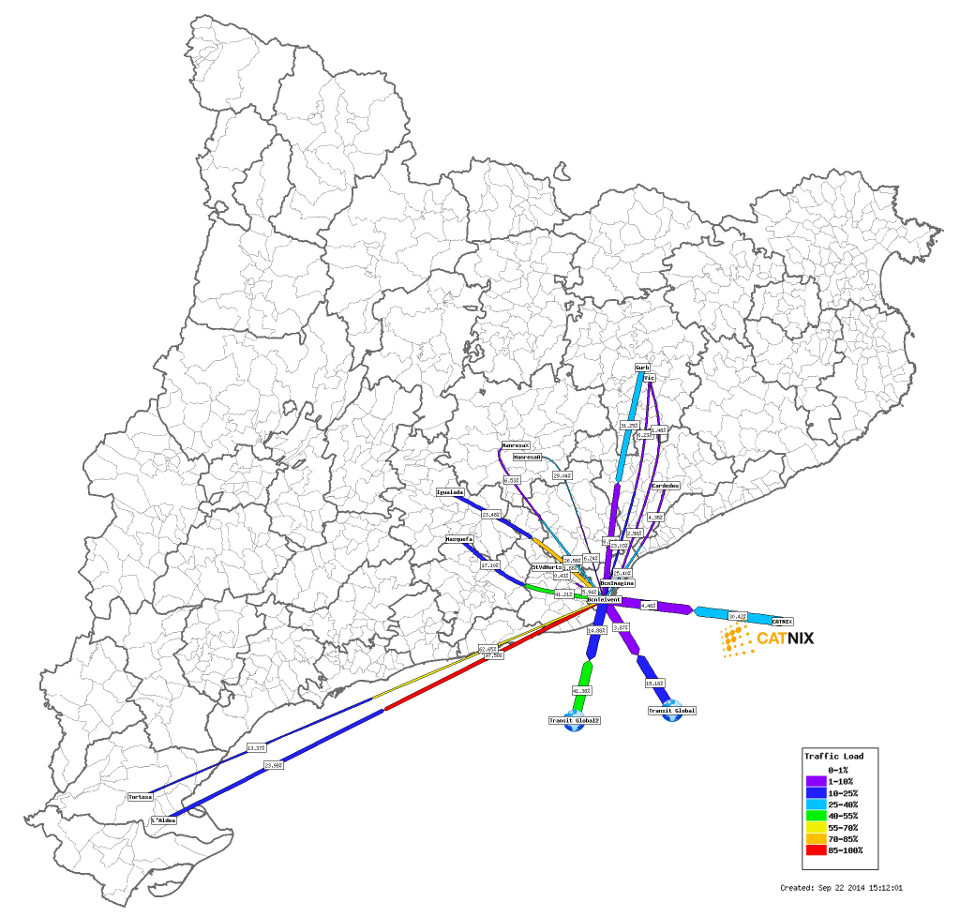
\includegraphics[width=0.95\linewidth]{sect3/figures/weathermap.jpg} 
  \caption[Guifi.net fiber POPs network map (Oct. 2014)]{Guifi.net fiber POPs network map (Oct. 2014).}
  \label{fig:pop_weathermap}
\end{figure}

With respect to the IXs operation, the following improvements have been applied during this year:
\begin{itemize}
  \item Economic compenstion system put in place (see report \emph{D.7.3.2 report on building support for BuB4Europe - b}) and already put in practice in 3 PoPs.
  \item Netflow feature activated in all core routers (part of the information needed to put the Economic compensation system in practice).
  \item A second carrier of 1Gb/s has been added to the alreay existing one in Telvent.
  \item Load balancing infrastructure to ensure maximum efficiency of the uplinks and redundancy put in place.
  \item Upgrade of Telvent's infrastructure to 10Gb/s
  \item A third IPv4 block obtained from RIPE-NCC
\end{itemize}

\figurename~\ref{fig:telvent_diagram} shows Telvent's PoP at wiring level after being reorganised and upgraded to 10Gb/s techology.

\begin{figure}[H]
  \centering
  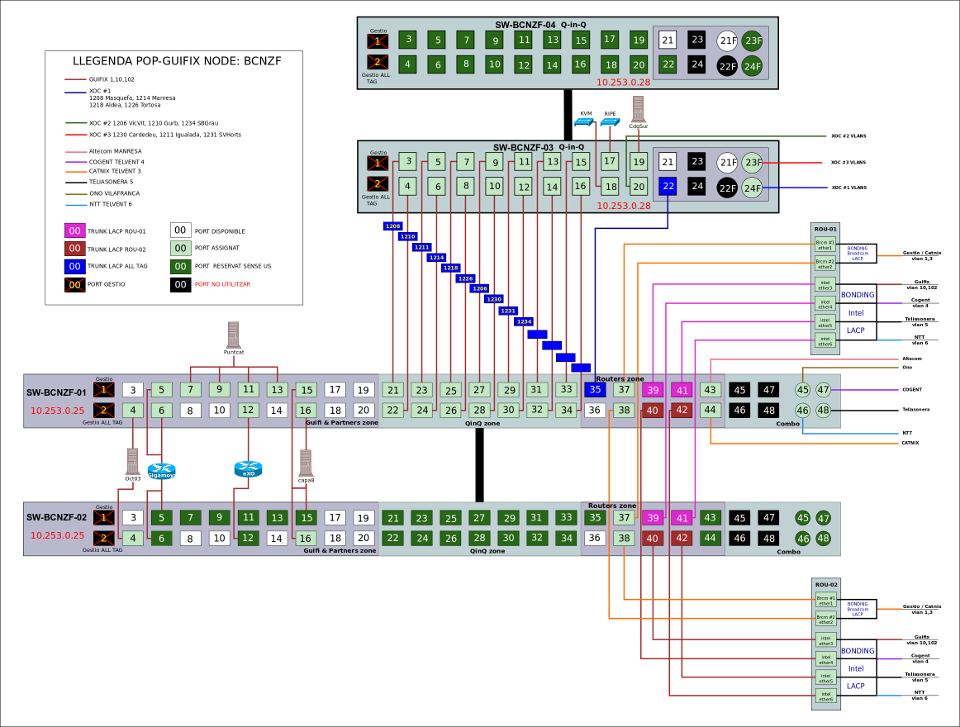
\includegraphics[width=0.95\linewidth]{sect3/figures/esquema_telvent_v14_3Novembre2014.png} 
  \caption[Telvent network diagram (Oct. 2014)]{Telvent network diagram (Oct. 2014).}
  \label{fig:telvent_diagram}
\end{figure}

During this period the number of peers at the CATNIX (the Catalan exchange point) has kept stable, but the traffic has steadely grown as \figurename~\ref{fig:catnix_transit} shows.

\begin{figure}[H]
  \centering
  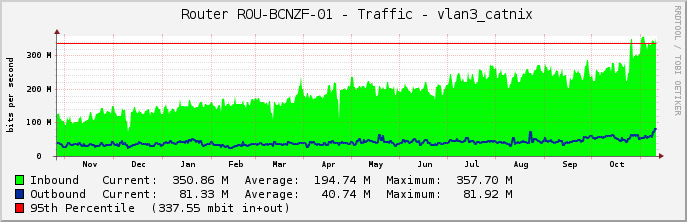
\includegraphics[width=0.95\linewidth]{sect3/figures/catnix.png} 
  \caption[CATNIX traffic 2014]{CATNIX traffic 2014.}
  \label{fig:catnix_transit}
\end{figure}

\figurename~\ref{fig:carriers_transit} shows the traffic of each carrier. As it can be observed he second carrier was activated in midMay. The effects of the load blancing can be observed from then on.

\begin{figure}[H]
  \centering
    \begin{tabular}{c}
      \resizebox{0.75\linewidth}{!}{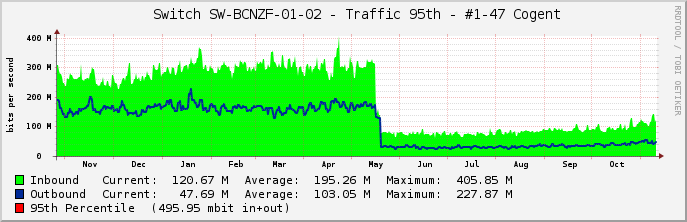
\includegraphics{sect3/figures/cogent.png}} \\
      \resizebox{0.75\linewidth}{!}{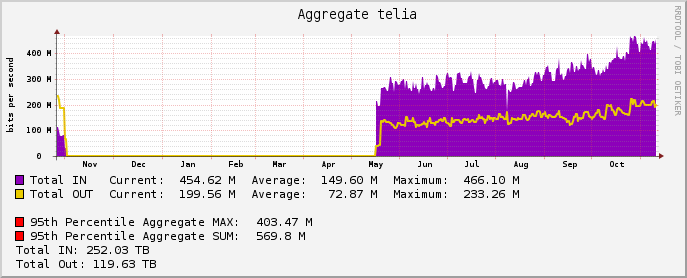
\includegraphics{sect3/figures/telia.png}} \\
    \end{tabular}
  \caption[Carriers traffic 2014]{Carries traffic 2014. Top: Cogent. Bottom: Telia.}
  \label{fig:carriers_transit}
\end{figure}

\figurename~\ref{fig:carriers_transit} shows the aggregated traffic of all guifi.net interconnections (the two carriers and the NIX) of the second week of November 2014. As it can be observed there are load peaks avobe 1.5Gb/s.

\begin{figure}[H]
  \centering
  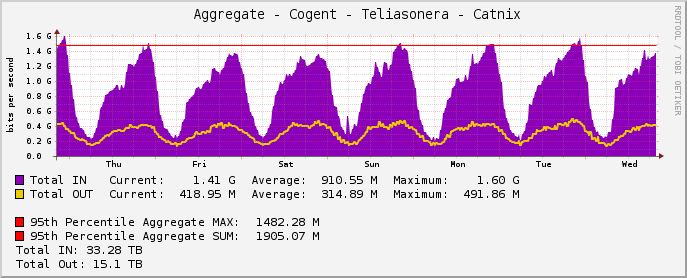
\includegraphics[width=0.95\linewidth]{sect3/figures/aggregated.png} 
  \caption[Interconnection - Total traffic Oct. 2014.]{Total interconnection inbond and outbound traffic Nov. 2014.}
  \label{fig:telia_transit}
\end{figure}


\FloatBarrier
\subsection{Pilot's POPs}
\label{pop_pilots}


\FloatBarrier
\subsubsection{Gurb}
\label{pop_gurb}

Operative since 2010, this year this PoP has been rebuilt to accommodate the hardware required for Gurb's OF pilot deployment and to install a new rack for servers. Firgure~\ref{fig:gurb_transit} shows the transit of this PoP in 2014.

\begin{figure}[H]
  \centering
  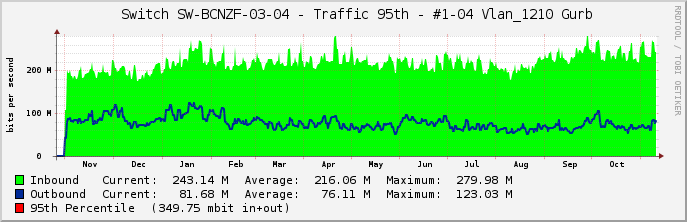
\includegraphics[width=0.95\linewidth]{sect3/figures/gurb.png} 
  \caption[Gurb PoP traffic 2014]{Gurb PoP traffic 2014.}
  \label{fig:gurb_transit}
\end{figure}


\FloatBarrier
\subsubsection{Vic}
\label{pop_vic}

This PoP, activated at the begining of the second reporting period, is allocated in a data centre of a premise of the local government (http://www.vitvic.cat/). Firgure~\ref{fig:vic_transit} shows the transit of this PoP 2014.

\begin{figure}[H]
  \centering
  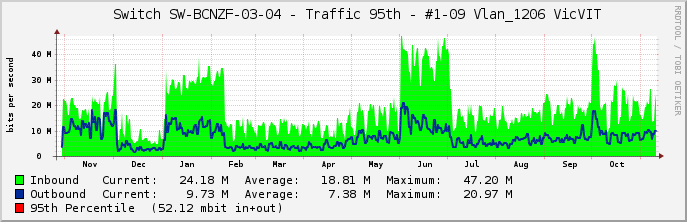
\includegraphics[width=0.95\linewidth]{sect3/figures/vic.png} 
  \caption[Vic PoP traffic 2014]{Vic PoP traffic 2014.}
  \label{fig:vic_transit}
\end{figure}


\FloatBarrier
\subsubsection{Rub\'{i}}
\label{pop_rubi}

This pilot's PoP has not been rised yet and it is not expected to be done shortly.


\FloatBarrier
\subsection{Other POPs}
\label{pop_others}

\figurename~\ref{fig:others_transit} shows the transit in 2014 of the rest of the operational territorial PoPs that were already active in 2013. As it can be observed, traffic has significantly incremented in all of them.

\begin{figure}[H]
  \centering
    \begin{tabular}{c}
      \resizebox{0.75\linewidth}{!}{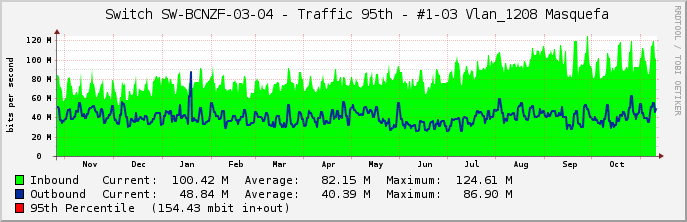
\includegraphics{sect3/figures/masquefa.png}} \\
      \resizebox{0.75\linewidth}{!}{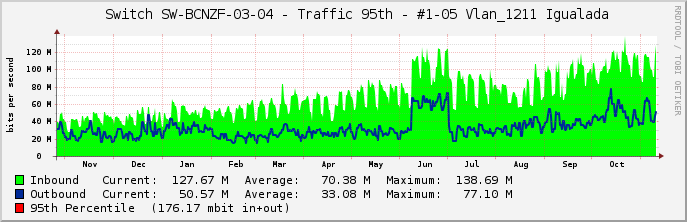
\includegraphics{sect3/figures/igualada.png}} \\
      \resizebox{0.75\linewidth}{!}{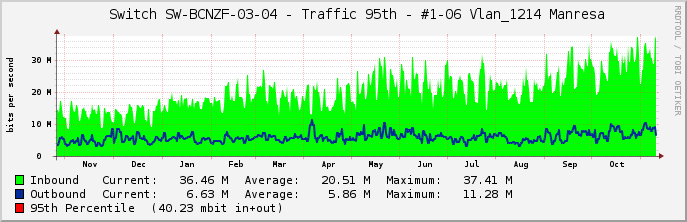
\includegraphics{sect3/figures/manresa.png}} \\
      \resizebox{0.75\linewidth}{!}{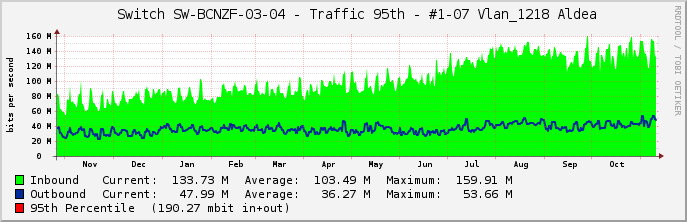
\includegraphics{sect3/figures/aldea.png}} \\
      \resizebox{0.75\linewidth}{!}{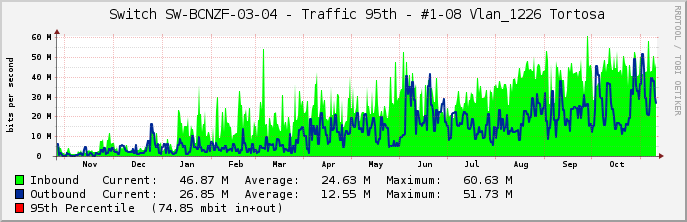
\includegraphics{sect3/figures/tortosa.png}} \\
    \end{tabular}
  \caption[Other PoPs traffic 2014]{Other PoPs traffic 2014. Top: Masquefa. Second top: Igualda. Middle: Manresa. Second bottom: Aldea. Bottom: Tortosa.}
  \label{fig:others_transit}
\end{figure}

